\documentclass[a4paper, 10pt]{article}
\usepackage[UTF8]{ctex}
\usepackage{geometry}
\geometry{left=3cm,right=3cm,top=3cm,bottom=3cm}
\usepackage{subfigure}
\usepackage[graphicx]{realboxes}
\begin{document}
  \title{实验报告:直流电桥测电阻}
  \author{郑志恒 2300012559}
  \maketitle
\section{实验设备}
电阻箱3个,指针式检流计,碳膜电位器,待测电阻3个,直流稳压电源,单刀双掷开关1个,双刀双掷开关1个,数字万用表1个,导线若干。

\section{实验原理}
\noindent 电桥平衡条件:
$$R_x=R_pR_1/R_2$$
只要知道了其余三个电阻的精确阻值,由电桥平衡条件就可以算出待测电阻的阻值。
\begin{figure}[ht]
    \centering 
    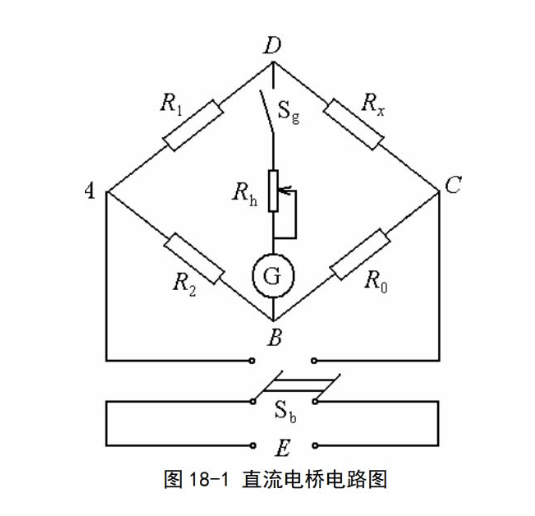
\includegraphics[height=9.3cm,width=10.5cm]{p1.png}
    
    \caption{fig1}
    \label{4}
    
    \end{figure}


\section{数据记录和处理}

\noindent 用万用表粗测电阻得到阻值约为$33\Omega$.
\begin{center}
    \begin{tabular}{|c|c|c|c|c|c|c|c|c|c|}
      \hline
      E/V&$R_h/\Omega$& $R_1/\Omega$ & $R_2/\Omega$ & $R_p/\Omega$&$R_p^\prime/\Omega$&$\Delta n$&$\Delta R_p/\Omega$&$R_x/\Omega$&S\\
      \hline
      2.0 &0 &100&100&33.7&33.8&6&0.1&33.7&2022\\
      \hline
      2.0 &0&100&1000&338.0&340.0&5&2.0&33.8&845\\
      \hline
      2.0 &0 &10k(A)&10k(B)&33.7&36.7&5&3.0&33.7&56.2\\
      \hline
      2.0 &0 &10k(B)&10k(A)&33.8&36.8&5&3.0&33.8&56.2\\
      \hline
      2.0 &3k &100&100&33.8&34.8&3&1.0&33.8&101.4\\
      \hline
      1.0 &0&100 &100&33.7&33.8&4&0.1&33.7&1348\\
      \hline
      

    \end{tabular}
  \end{center}

\noindent 定义电桥灵敏度$S=\frac{\Delta n}{\frac{\Delta R_x}{R_x}}$,表示电桥平衡后,$R_x$的相对该变量所引起的检流计偏转的格数。具体测量时$\frac{\Delta R_0}{R_0}$可以代替$\frac{\Delta R_x}{R_x}$.由该公式可以计算出不同情况下电桥的灵敏度如表所示。

\noindent  由交换臂法得到的电阻阻值为:
$$R_x=\sqrt{33.7\times 33.8}=33.75\Omega$$

\noindent 不确定度分析:
$$\sigma_{R_1}=\sigma_{R_2}=e/\sqrt{3}=\frac{10k\times 0.1\%}{\sqrt{3}}=5.773\Omega$$

$$\sigma_{R_p}=e/\sqrt{3}=\frac{30\times 0.1\%+3\times 0.5\%+0.8\times 2\%}{\sqrt{3}}=0.035\Omega$$

$$\delta R_x=\frac{0.2\Delta R_x}{\Delta n}=0.12\Omega$$

\noindent 故有:
$$\sigma_{R_x}=[(\delta R_x)^2+(\frac{R_p}{R_2})^2\sigma_{R_1}^2+(\frac{R_pR_1}{R_2^2})^2\sigma_{R_2}^2+(\frac{R_1}{R_2})^2\sigma_{R_p}^2]^{1/2}=0.128\Omega$$

\noindent 测量结果为:
$$R_x=(33.75\pm0.128)\Omega$$

\section{分析与讨论}
\noindent \textbf{如何提高电桥测量电阻的精度?}

\noindent i.可以通过选用更高灵敏度的检流计,由电桥灵敏度公式:
$$S=\frac{S_iE}{R_1+R_2+R_p+R_x+R_g(2+R_1/R_x+R_p/R_2)}$$
通过提高检流计的灵敏度可以提高电桥的灵敏度或提高检测电压,从而实现更精准的测量。

\noindent ii.可以通过适当减小$R_1$和$R_2$来提高电桥灵敏度,以实现更精准的测量

\noindent iii.采用四线法测量可以抵消测试引线电阻的影响,提高测量精度.








\end{document}